\section{System Architecture}

\paragraph{}
Operating Systems for Embedded Devices started appearing in the 00's.
Since then design choices have evolved with the technology, reseach and trends.
\\
In this section, we'll explain the different kernel architectures commonly found in RTOS's and their impact on the operating system.

%\subsection{Base concepts}

%\paragraph{}
%Beforehand, we'll have to explain (or remind) some technical terms in order for the reader to fully understand this chapter.

\subsection{Kernel}
\paragraph{}
The kernel is the center piece of an operating system.
The role of the kernel is to manage every critical function of an operating system.
It could technically run by itself but it wouldn't be very practical.
An operating system is built around its kernel and in the case of an RTOS, kernel design is critical for ensuring strict deadlines.
The tasks a kernel usually manages consists of:
\begin{itemize}
    \item memory management
    \item process and CPU scheduler
    \item device drivers
    \item system calls
\end{itemize}


\subsection{User space and kernel space}
\paragraph{}
Almost every operating system makes the distinction between user space and kernel space.
The memory allowed to the operating system is divided into two distinct segments.
The goal is to provide memory and hardware protection against malicious or faulty behaviors.

The first one, the kernel space, is dedicated to operations the closest to the hardware.
It is reserved for the most trusted operations of the operating system.
Due to its central position in the operating system, any bug in the kernel can lead to system failure.
In order for an user process to use the hardware, it needs to ask the kernel through an API so that the kernel performs the operation for the process.

The second one, the user space is dedicated to all the code running outside of the kernel-space such as applications, programs and libraries.
Each user-space process has its own memory space and cannot access the memory of another process (unless they use shared memory).

\subsection{CPU modes}
%https://minnie.tuhs.org/CompArch/Lectures/week07.html
%https://blog.codinghorror.com/understanding-user-and-kernel-mode/
\paragraph{}
CPU's run on different operating modes (also called states or levels).
In kernel mode (also called privilege mode or unrestricted mode), the CPU may perform any operation without restriction.
In user mode, direct access to hardware is prohibited.

Those modes prevent the application software from accessing the hardware directly.
Applications are resetricted to their address space 
    and should use the operating system's abstract services in order to perform operations on the hardware.

\subsection{Interprocess communication}
%https://www.geeksforgeeks.org/interprocess-communication-methods/
\paragraph{}
Interprocess communication (IPC) designates the mechanisms used to share data between processes in an operating system.
Those mechanisms can differ from OS to OS but are generally the same.
We can notably cite:
\begin{itemize}
    \item Pipes
    \item Names Pipes
    \item Message Queuing
    \item Semaphores
    \item Shared memory
    \item Sockets
\end{itemize}

\subsection{Interrupt}
\paragraph{}
An interrupt is a signal emitted by hardware or software to the CPU signaling an event.
When an interrupt happens, the state of the current program is saved 
    and the routine related to the interrupt is executed.

The origin of an interrupt can be of all sort, 
    from changing running thread in a single core processor to pressing a key in a keyboard.

\subsection{Kernel Architecture}

\subsubsection{Monolithic architecture}
% Explanation
A monolithic kernel is composed of a single block of code running a single large process.
Thanks to its simplicity, fast execution time and low memory footprint, it served as the norm for early RTOS's.
In monolithic systems, the operating system runs as a whole in privilege mode.
The application built upon it requests services by calling \textit{system call} instructions.

% TODO paragraph too complex
% Example?
% Interrupt handling
Interrupt handling is performed directly in the kernel for the most part and interrupt handlers are not full-fledged processes.
Consequently, the interrupt handling overhead is very small because there is no full task switching when triggered
    but the handling code cannot invoke most system services like blocking synchronization primitives.
Instead of that, the scheduler is disabled during the Interrupt Service Routine (ISR) and only hardware prioritization is in effect.
Hence, the ISR is implicitly executed at higher priority than all the other tasks of the system.

% Advantages
The monolithic kernel architecture is comparatively quite fast, since ev\-ery\-thing is implemented under the same address space.
% Disadvantages
Nonetheless, due to its design, it is prompt to critical failures, difficult to understand, maintain and update.

\subsubsection{Micro-kernel architecture}
%Explanation
In a micro-kernel architecture, the kernel is broken down into separate processes;
     the \texttt{micro-kernel}, a minimalistic kernel;
     and the \texttt{servers}, extending the functionalities of the said microkernel.

The servers functionalities are often features of the kernel that can run in the user space
    rather than the kernel space (such as the file system, network features or device access).
A message-passing communication mechanism is used to communicate between the kernel and the servers.
The main purpose of the microkernel is to handle the communication between the application and the servers
    and to perform the critical operations (such as accessing I/O device registers) that would be difficult or inefficient to perform in user-space.

% Interrupt handling
Interrupt requests are handled by transforming them into messages to the appropriate handling task.
The interrupt handler runs in interrupt service mode and performs the work required by the hardware, then sends a message to an interrupt service task
Interrupt service tasks operate like any other task, including the blocking primitives.
The overhead of interrupt handling is higher than with the monolithic architecture since it implies a full task switch.

% Advantages
A micro-kernel architecture is considered more secure, as kernel-space functionalities and user-space functionalities are dissociated.
It is also more reliable and resilient as if a server crashes, it does not stop the microkernel from running nor the others servers.
The memory footprint can also be minimized since we can choose which server we want to use and only boot with those.
From a maintainer point of view, it is also less complex, easier to understand and update.
% Disadvantages? more sys calls, slower due to IPC
The micro-kernel architecture needs an inter-process communication (IPC).
A message-passing mechanism has to be used and is inheritantly slower than a direct function calls.
\\

\begin{figure}[!h]
    \centering
    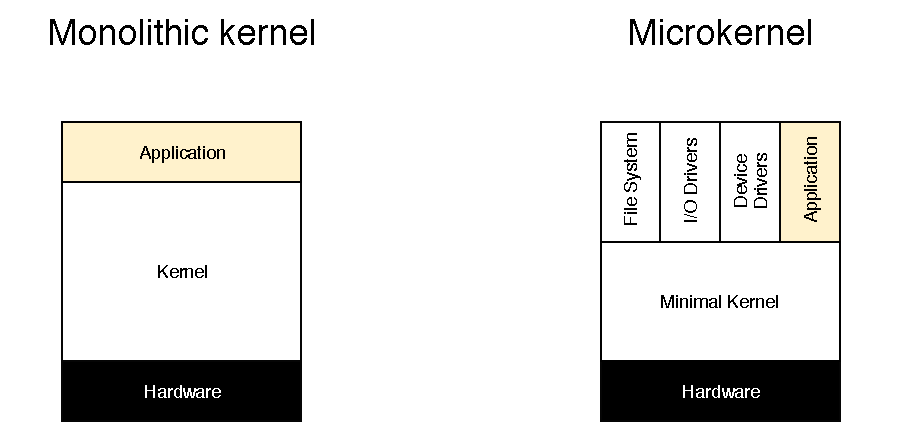
\includegraphics[scale=0.7]{assets/kernel_types.pdf}
    \caption{\label{fig:kernel-types}Different kernel designs}
\end{figure}

% Others architectures
% Complete by mentioning other types?
Of course there are more architectures than what is listed above as it is far from exhaustive.
But in the context of this thesis, we considered that explaining in detail each one would not be relevant.
The two designs presented are the most common and provide a good glance at what a kernel looks like.
Also, the following parts of this thesis will expand on this
    and we'll see in practise what each RTOS takes from this theoretical point of view.
